\documentclass[12pt,a4paper]{article}
%\usepackage{natbib}         % Pour la bibliographie
\usepackage{url}            % Pour citer les adresses web
\usepackage[T1]{fontenc}    % Encodage des accents
\usepackage[utf8]{inputenc} % Lui aussi
\usepackage[frenchb]{babel} % Pour la traduction française
\usepackage{numprint}       % Histoire que les chiffres soient bien

\usepackage{amsmath}        % La base pour les maths
\usepackage{mathrsfs}       % Quelques symboles supplémentaires
\usepackage{amssymb}        % encore des symboles.
\usepackage{amsfonts}       % Des fontes, eg pour \mathbb.

\usepackage[svgnames]{xcolor} % De la couleur
\usepackage{geometry}       % Gérer correctement la taille

%%% Si jamais vous voulez changer de police: décommentez les trois 
%\usepackage{tgpagella}
%\usepackage{tgadventor}
%\usepackage{inconsolata}

%%% Pour L'utilisation de Python
\usepackage{pythontex}

\usepackage{graphicx} % inclusion des graphiques
\usepackage{wrapfig}  % Dessins dans le texte.

\usepackage{tikz}     % Un package pour les dessins (utilisé pour l'environnement {code})
\usepackage[framemethod=TikZ]{mdframed}
% Un environnement pour bien présenter le code informatique
\newenvironment{code}{%
\begin{mdframed}[linecolor=Green,innerrightmargin=30pt,innerleftmargin=30pt,
backgroundcolor=Black!5,
skipabove=10pt,skipbelow=10pt,roundcorner=5pt,
splitbottomskip=6pt,splittopskip=12pt]
}{%
\end{mdframed}
}

\newcounter{byear}
\setcounter{byear}{\the\year}
\addtocounter{byear}{-1}

% Mettez votre titre et votre nom ci-après
\title{Mise en Cohérence des Objectifs de TIPE (MCOT) \\
Modélisation et Prévision \\
du risque de cambriolage en ville}
\author{Maxime MUNIER, MPI\oldstylenums{}, \oldstylenums{\arabic{byear}}-\oldstylenums{\the\year} }
%% À décommenter si vous ne voulez pas que la date apparaisse explicitement
\date{}

% Un raccourci pour composer les unités correctement (en droit)
% Exemple: $v = 10\U{m.s^{-1}}$
\newcommand{\U}[1]{~\mathrm{#1}}

% Pour discuter avec le prof dans le document: le premier argument est 
% le nom de celui qui fait la remarque et le second la remarque 
% proprement dite: \question{jj}{Que voulez-vous dire par là ?}
% \reponse{Droopy}{I'm very happy...}
\usepackage{todonotes}
\newcommand{\question}[2]{\todo[inline,author=#1]{#2}}
\newcommand{\reponse}[2]{\todo[inline,color=green,author=#1]{#2}}

% Les guillemets \ofg{par exemple}
\newcommand{\ofg}[1]{\og{}#1\fg{}}
% Le d des dérivées doit être droit: \frac{\dd x}{\dd t}
\newcommand{\dd}{\text{d}}



% NB: le script TeXcount permet de compter les mots utilisés dans chaque section d'un document LaTeX. Vous en trouverez une version en ligne à l'adresse
% http://app.uio.no/ifi/texcount/online.php
% Il suffit d'y copier l'ensemble du présent document (via Ctrl-A/Ctrl-C puis Ctrl-V dans la fenêtre idoine) pour obtenir le récapitulatif tout en bas de la page qui s'ouvre alors.

% Pour récupérer les bonnes entrées bibliographiques, je vous conseille l'usage de scholar.google.fr pour les recherches
% et la récupération des entrée BibTeX comme décrit dans cette vidéo: https://www.youtube.com/watch?v=X-9T2Oaj-5A

\newcommand{\positionnementThematique}[1]{
\section*{Positionnement thématique}
{\it #1}}

\newcommand{\motclefs}[2]{
\section*{Mots-clefs}
\begin{description}
\item[Mots-clefs] -- #1 
\item[Keywords]   -- #2
\end{description}
}

\geometry{
a4paper, 
total={150mm, 257mm},
left=30mm,
top=20mm,
}

\begin{document}

\maketitle

\positionnementThematique{INFORMATIQUE (informatique pratique), MATHEMATIQUES (Probabilités)}

\motclefs{Cambriolage -- Modélisation -- Prévision -- Algorithme -- Séisme}{Heist -- Modeling -- Expectation -- Algorithm -- Earthquake}


\section*{Bibliographie commentée}
% D'après TeXcount, la section fait 366 mots: 
% 366+3+0 (1/0/4/0) Section: État de l'art

%\begin{wrapfigure}[8]{r}{0.5\linewidth}
%\vspace*{-2\baselineskip}
%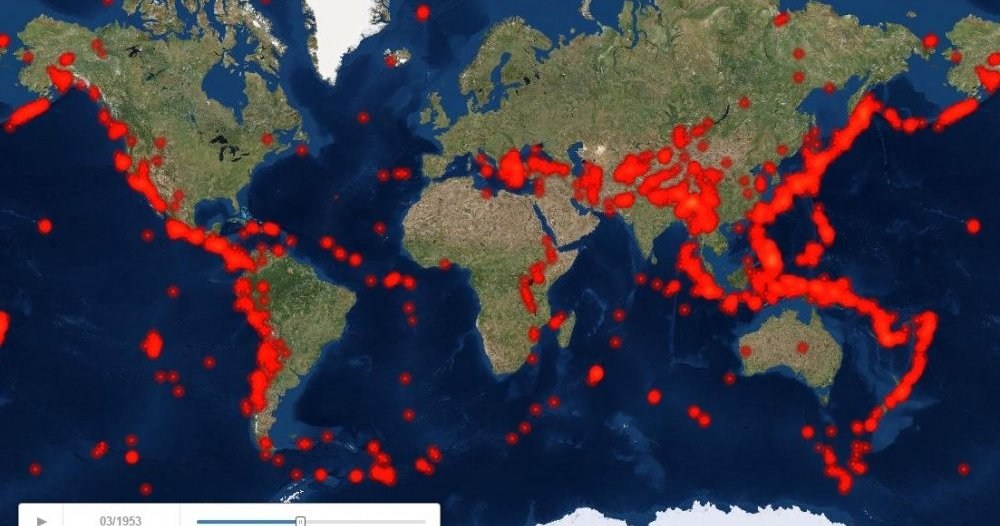
\includegraphics[width=\linewidth]{Fig01}
%\end{wrapfigure}
La prédiction policière \cite{Predic} est un domaine de recherche dont l’objectif principal est de développer des machines à prédire les crimes, en tirant profit des algorithmes et de l’accessibilité croissante à une diversité de données. Depuis 2011, l’enthousiasme autour de « Predpol » \cite{Lemonde}, le logiciel de police prédictive américain, électrise la terre entière. Son algorithme secret, toujours comparé aux précogs de « Minority Report » ou à la Machine de « Person of Interest » \cite{Interstices}, semble tenir plus de la magie que de la science. La société, elle, affiche partout des résultats là où sa technologie est déployée dans des villes américaines comme Los Angeles et Atlanta où l'on y observe une baisse de la criminalité de 10 à 30\%. 





Depuis quelques années, Andrea Bertozzi \cite{Berto}, anime un groupe de chercheurs rassemblant mathématiciens, anthropologues et policiers. Leur but est de comprendre et prévenir l’activité criminelle dans une ville comme Los Angeles. Andrea Bertozzi a vite compris que les systèmes criminels pouvaient être modélisés à l'aide de ses outils favoris : la densité criminelle d'un lieu ayant tendance à alimenter son potentiel criminel, et réciproquement, chaque donnée évolue en fonction de l'autre. Chez les malfrats, on a tendance à se rapprocher peu à peu des zones les plus attractives en matière de criminalité... Ce qui finit par faire augmenter le nombre de crimes commis dans ces zones, et donc par faire augmenter leur attractivité. Pour tenter de comprendre où et quand pourraient se dérouler les prochains crimes, la mathématicienne et son équipe ont pris en compte un certain nombre de paramètres qui seraient liés à un concept connu sous le nom de « théorie de la vitre brisée » \cite{Vitres} qui se base sur le principe suivant : si une vitre brisée n'est pas immédiatement réparée, il est probable que d'autres vitres du même bâtiment seront bientôt brisées à leur tour, le lieu étant considéré comme abandonné et délabré. Un principe qui fonctionne aussi avec une maison cambriolée qui, parce qu'elle est identifiée comme insuffisamment protégée, a plus de chances de l'être à nouveau. D'un point de vue purement mathématique, l'équipe de recherche en est venue à la conclusion suivante : de par leur structure, les équations obtenues rappellent celles qui modélisent l'évolution de certaines bactéries. Bertozzi voit du même œil la répartition et l'évolution de la criminalité : un crime non signalé, non élucidé ou non puni peut servir d'origine à la constitution progressive d'un « point chaud », une zone géographique dans laquelle les crimes seront de plus en plus nombreux. La dynamique des tremblements de terre et de leurs répliques semble également très proche de la façon dont un crime peut être suivi par d'autres, au même endroit ou dans les environs.

C’est ce lien avec la sismologie en particulier qui semble relativement intéressant \cite{Youtube}. En effet, on pourrait croire que les tremblements de terre sont aléatoires et distribués selon le modèle de Poisson de sorte que chaque tremblement de terre soit indépendant des autres. Mais en réalité, s’il y a un tremblement de terre, il va très probablement y avoir des contrecoups, c’est-à-dire une série de tremblements de terre, au même endroit, en succession rapide. Les scientifiques et les mathématiciens ont développé le « Processus de Hawkes » \cite{Hawkes} qui prend en compte le fait que des évènements ne sont pas complètement indépendants les uns des autres. Ce qui est intéressant, c’est que la criminalité, se base sur le même schéma \cite{Risque}. Si l'on considère les cambriolages, les personnes qui se sont déjà faites cambriolés savent que les chances de se faire cambrioler à nouveau dans une courte période de temps, sont beaucoup plus fortes. Plusieurs raisons peuvent expliquer cela: les cambrioleurs connaissent déjà le plan de la maison, ils savent où sont gardés les objets précieux, ils ont des informations sur le quartier. Ainsi, les chances de se faire cambrioler à nouveau augmentent, mais elles augmentent aussi pour les voisins, les voisins des voisins, et ainsi de suite dans toute la rue. Ce processus qui considère les évènements comme liés dans le temps, veut dire qu’on peut modéliser ce qui se passe avec les cambriolages de façon statistique. 


\section*{Problématique retenue}

A l’aide de modèles sismiques et de données du passé recensées, peut-on réussir à modéliser et prédire le risque de cambriolages en ville?

\section*{Objectifs du TIPE}

\begin{enumerate}
    
	\item	Modélisation: après quelques rappels théoriques, j'expliciterai le "Processus de Hawkes" ainsi que le modèle utilisé pour répondre à la problématique du sujet.
    
    \item	Simulation: En se basant sur la base de données criminelle de Chicago, j'estimerai les paramètres du modèle à l'aide de plusieurs méthodes et algorithmes utilisées en statistiques.
    
    \item	Validations et Observations: En utilisant les bases de données des différentes années, il sera assez facile de comparer les estimations du modèles ainsi conçu avec les données de la réalité afin de valider ou non ce modèle mathématiques. Des commentaires sur les résultats seront également exprimés.
    
\end{enumerate}

% Pour faire apparaître la bibliographie avec des chiffres, 
% dans l'ordre d'apparition dans le texte
\bibliographystyle{unsrt-fr}     % Style de la bibliographie (numérotée dans l'ordre d'apparition du texte)
\bibliography{biblio} % Nom du fichier .bib à utiliser


\end{document}